\documentclass[]{article}

\usepackage{amsmath}
\usepackage{float}
\usepackage{graphicx}
\usepackage[margin=1in, paperwidth=8.5in, paperheight=11in]{geometry}

%opening
\title{Neural Networks: An Exploration}
\author{Patrick Huston, David Abrahams, Philip Seger}

\begin{document}

\maketitle

\begin{abstract}

\end{abstract}

\section{What is a Neural Network?}

A Neural Network is a machine learning model roughly based on the makeup of the brain. A NN is comprised of a series of \textbf{layers}. Each of these layers is comprised of \textbf{neurons}. Each neuron has an output, known as an \textbf{activation}, which is simply a linear combination of the outputs (activations) of the previous layers.

The connections between the neurons are often called \textbf{synapses}. Each synapse has an associated value which is the coefficient in the linear combination that produces the neurons in the next layer. The associated values of all the synapses between two layers comprise a \textbf{weight matrix}.

\section{Making Predictions}

Above we have simple neural network, which takes in two inputs (features), and returns one output (prediction). Let's assume we have 3 samples. This means X is a 3x2 matrix. $W_1$ is a matrix of synapse coefficients. We can see that there are four synapses between the first two layers. $W_1$ is a 2x2 matrix, where each row corresponds to the synapses coming out of one of the input neurons.

\begin{figure}[H]
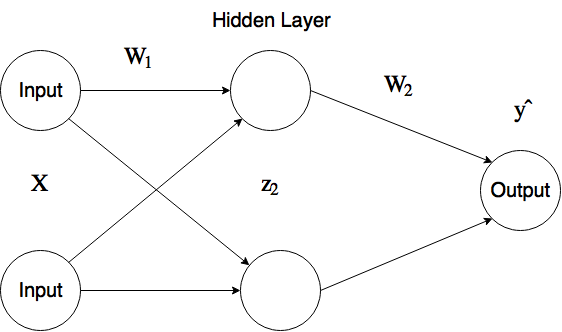
\includegraphics[width=4in]{neuralnet.png}
\centering
\end{figure}

In this neural net:

\begin{align}
	z_2 &= X W_1\\
	\hat{y} &= z_2 W_2
\end{align}

\section{Activation functions}

Perhaps at this point you have astutely observed that currently our Neural Network is basically just a linear regression model, since the output is a linear combination of the inputs. It's time to introduce one of the most important features of neural networks: \textbf{nonlinearity}. Most neural network layers apply a activation function to their activations before passing on their output to the next layer. This transformed activation is known as the layer \textbf{activity}. All we have to do to make our network capable of predicting nonlinear relationships is update our equations:

\begin{align}
	a_2 &= \tanh (z_2) \\
	\hat{y} &= a_2 W_2
\end{align}

The hyperbolic tangent function scales each activation from -1 to 1. We're done! This is now a neural net capable of making predictions.

\begin{figure}[H]
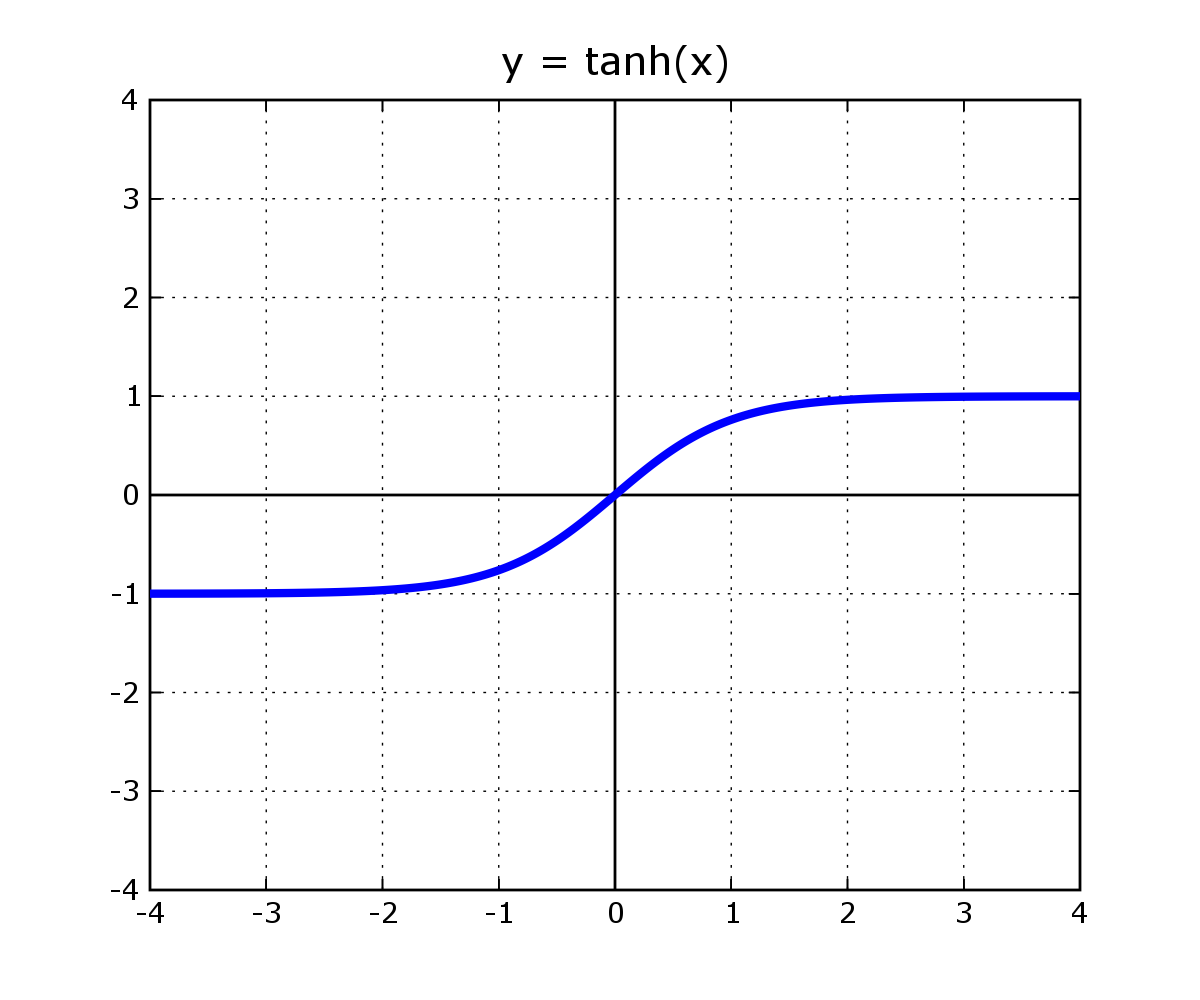
\includegraphics[width=4in]{tanh.png}
\centering
\end{figure}


\section{Training a Neural Network}

Making predictions with NNs is great, but it's not worth much unless we can improve our predictions. Gradient descent to the rescue!

\subsection{Gradient Descent and Neural Networks}
With random weights, a NN is pretty terrible at making predictions. To improve our model, we first need to quantify exactly how wrong our predictions are. We'll do this with a cost function. A cost function allows us to express exactly how wrong or "costly" our models is, given our examples.

A common way to compute an overall cost is to take each error value, square it, and sum the values.

\begin{equation}
	J = \Sigma \frac{1}{2}(y- \hat{y})^{2}
\end{equation}

This cost is a function of two things - the input data, and the weights on the synapses. We can't change the data, so we'll improve the accuracy by modifying the weights!

Conceptually, what we'll be doing is computing derivative of the cost with respect to each weight matrix. We'll use these derivatives to compile a gradient, which we can then use to change the weights incrementally as our network improves!


\subsection{Applying Gradient Descent to Train a Network}
Let's get to applying gradient descent to improve and train a neural network. Assuming we have a network with one hidden layer and according weight matrices $W_1$ and $W_2$.

We need some way to compute $\frac{\partial J}{\partial W}$. Because we have two weight matrices, we'll have to split the computations up into $\frac{\partial J}{\partial W_2}$ and $\frac{\partial J}{\partial W_1}$ - the partial derivatives of the cost $J$ with respect to the weight matrices $W_1$ and $W_2$. For ease, we'll start with $\frac{\partial J}{\partial W_2}$.

\subsubsection{$\frac{\partial J}{\partial W_2}$}

We'll start with this expression -

\begin{equation}
	\frac{\partial J}{\partial W_2} = \frac{\partial \sum \frac{1}{2}(y-\hat{y})^2}{\partial W_2}
\end{equation}

Taking the derivative of this expression (temporarily setting aside the summation) simply involves a lot of chain rule. Backpropagation - don't stop doing the chain rule, ever.

The first step looks like this:

\begin{equation}
\frac{\partial J}{\partial W_2} = -(y-\hat{y}) \frac{\partial \hat{y}}{\partial W_2}
\end{equation}

Next, we'll expand $\frac{\partial \hat{y}}{\partial W_2}$. This step is actually really easy, because $\hat{y}$ is simply a scalar multiple of $W_2$!

\begin{align}
\hat{y} &= a_2 W_2 \\
\frac{\partial \hat{y}}{\partial W_2} &= a_2 \\
\frac{\partial J}{\partial W_2} &= - a_2^T (y-\hat{y})
\end{align}

There we have our final equation for $\frac{\partial J}{\partial W_2}$! A way to think about what's going on here is that we're "backpropagating" the error to each weight. The neurons with larger activities will contribute more to the error, and therefore the synapses connected to them will have larger $\frac{\partial J}{\partial W_2}$s. The synapses connecting the most active neurons' weights will be changed most when we perform gradient descent.

To find the rate of change of $\hat{y}$ with respect to $z_3$, we need to differentiate the activation function with respect to $z$. Once we compute that, we can now replace $\frac{\partial \hat{y}}{\partial z^{(3)}}$ with $f^\prime(z^{3})$

\begin{equation}
\frac{\partial z^{(3)}}{\partial W_2}=
-(y-\hat{y}) f^\prime(z^{(3)}) \frac{\partial z^{(3)}}{\partial W_2}
\end{equation}

Finally, we need to investigate the relationship between $z^{(3)}$ and $W^({2})$. If we take a look at a previous equation describing the derivation of the activation, we get $z^{(3)} = a^{(2)}W_2$. It's just a linear relationship!

Applying this, we get to the final equations:

\begin{equation}
\frac{\partial J}{\partial W_2} =
(a^{(2)})^T\delta^{(3)}\tag{6}
\end{equation}

where

\begin{equation}
\delta^{(3)} = -(y-\hat{y}) f^\prime(z^{(3)})
\end{equation}

\subsubsection{$\frac{\partial J}{\partial W_1}$}

We have one more derivative to compute - $\frac{\partial J}{\partial W_1}$. The process for this derivative starts the same as described above, but with an additional application of the chain rule to back-propagate error through each layer. The final equation begins with:

\begin{align}
	\frac{\partial J}{\partial W_1} &= \frac{\partial \sum \frac{1}{2}(y-\hat{y})^2}{\partial W_1} \\
	\frac{\partial J}{\partial W_1} &= -(y-\hat{y}) \frac{\partial \hat{y}}{\partial W_1}
\end{align}

To find $\frac{\partial \hat{y}}{\partial W_1}$, we must first investigate the relationship between $\hat{y}$ and $a_2$.

\begin{align}
	\frac{\partial J}{\partial W_1} &= -(y-\hat{y}) \frac{\partial \hat{y}}{\partial a_2} \frac{\partial a_2}{\partial W_1}
\end{align}

Something fascinating happens here. Similar to earlier, because $\hat{y}$ is a scalar multiple of $a_2$ and $W_2$:

\begin{align}
	\frac{\partial \hat{y}}{\partial a_2} = W_2
\end{align}

Now we continue and separate $\frac{\partial a_2}{\partial W_1}$.

\begin{align}
	\frac{\partial a_2}{\partial W_1} &= \frac{\partial a_2}{\partial z_2} \frac{\partial z_2}{\partial W_1}
\end{align}

To find $\frac{\partial a_2}{\partial z_2}$, we have to differentiate the activation function with respect to $z$. Once we compute that, we can now replace $\frac{\partial a_2}{\partial z_2}$ with $\tanh^\prime(z_2)$:

\begin{align}
	\frac{\partial a_2}{\partial z_2} &= \tanh^\prime(z_2)
\end{align}

Finally, we differentiate $z_2$ with respect to $W_1$. It's just another linear relationship!

\begin{align}
	\frac{\partial z_2}{\partial W_1} &= X
\end{align}

We now have all the pieces for $\frac{\partial J}{\partial W_1}$. Putting it all together:

\begin{align}
\frac{\partial J}{\partial W_1} =
- X^{T}
(y - \hat{y})
W_2^{T}
\tanh^\prime(z_2)
\end{align}

\section{LSTMs}

NNs have another fascinating use case. They are also able to learn patterns in sequential data. A neural network that learns sequential data is known as a \textbf{Recurrent Neural Network}. The only difference is that at each time step, the hidden layer receives the hidden layer from the previous timestep as an input.

  LSTM3-SimpleRNN.png
A downside to this basic implementation is the fact that the network quickly forgets information from several timesteps ago. To overcome this, many people use a special implementation of an RNN known as an LSTM (long short-term memory) network.

  LSTM3-var-GRU.png
  LSTM2-notation.png

LSTMs rely on a \textbf{cell state}: the horizontal line running through each timestep. This line is like a "conveyor belt," carrying information across timesteps. The information that is stored or changed on the cell state is dictated by a forget gate. In short, the network learns what to remember, and what to forget.

\section{Implementations}

\subsection{Predicting the Weather}

One of the neural net implementations we did was training and then running a time-series of daily weather data through a LSTM. Our results were okay (better than a simple baseline model, but not much better). Here's a snapshot of our model's output, after being trained on 14-day sliding windows of weather data.

\subsection{Text Generation using an LSTM Network}
Another neural net implementation we explored was a character-level NLP LSTM network. We trained the network on several different books from Project Gutenberg. Below are some outputs of the network at the later stages of training. Note that we used a seed text of 'The quick brown fox jumps' to give the network a starting point to generate from.

"The quick brown fox jumpstence in his friends. The unaveruaties of the period of the family were in town, before I feet the state of his concern, and was as for a man every dear friends in minet seeing the lady for shem allow..."

"The quick brown fox jumpst to be affectionate supposition than he was the compliment of she seemed of her father and more certain that he was not so well groding to ask you, I would not contrive to her as to the particulars o..."

"The quick brown fox jumpster, the children which his advice, as he had been so fortunate as to be dinner with him to say that his addressing with the matter; and the evening, however, soon afterwards in their character, she s..."

\end{document}
